% !Mode:: "TeX:UTF-8"

\chapter[MPI简介]{MPI简介}
\section{MPI概要介绍}
MPI的全称为Message Passing Interface,是目前比较流行的一种基于消息传递的并行编程模型,而不是一种程序设计语言,MPI可以与广为使用的Fortran和C/C++语言进行绑定,并且支持多种硬件平台和各种操作系统。

来自美国和欧洲的60多人,属于40多个不同单位和组织对MPI标准付出了努力。其中包括多数并行计算机的主要生产商,大学的研究人员
、科研机构,科研应用部门。

有关的工作及其组织包括 Venus (IBM)、 NX/2 (Intel)、 Express (Parasoft)、 Vertex (nCUBE) 、P4 (ANL)、 PARMACS (ANL) ,还包括Zipcode (MSU)、 Chimp (Edinburgh University) 、PVM (ORNL, UTK, Emory U.) 、Chameleon (ANL) 、PICL (ANL)等。

1992年4月29日至30日,在威吉尼亚的威廉姆斯堡召开的分布存储环境中消息传递标准的讨论会举办,讨论MPI的标准化工作。最终由Dongarra,Hempel,
Hey和Walker提出的建议初始草案于1992年11月推出,随后在次年2月完成了修订,也就是众人熟知的MPI1.0。之后,为一个称为MPI论坛的非官方组织应
运而生,论坛对MPI标准的发展和成熟的促进起到了至关重要的作用。

1995年6月,新版本MPI1.1推出,在MPI1.0的基础上作了进一步的修改、完善和提高。但是当初推出MPI标准时,为了能够使MPI被快速实现和接受
,许多重要但复杂的功能接口都没有定义。在MPI被接受之后,提高MPI功能和完善复杂功能的要求就凸显重要性。接下来,在1997年的7月,
推出了MPI的扩充版本MPI-2,之前的MPI各种版本统称为MPI-1。MPI-2的改进了很多功能,扩充了很多接口,主要是三个方面:并行I/O、
远程存储访问和动态进程管理。

\subsection{MPI定义}
MPI有多种定义,主要分为3种,这3种定义很好地阐述了MPI的本质和作用。

\begin{enumerate}
\item MPI是一个并行标准库,不是一门计算机程序语言。把MPI当成独立的并行编程语言是不准确的。但
是可以按照语言的不同,实现MPI与各个编程语言的结合,可以把FORTRAN搭配MPI或C搭配MPI,作
可以理解为原串行语言基础添加了MPI扩展库之后形成的新的并行语言。现在,MPI库可以被FORTRAN77/C/Fortran90/C++调用,
从语法上讲它遵守所有特定语言对库函数/过程的语法规则,等同于常见的函数调用和语言语法.
\item MPI做为并行计算的标准或规范的代表,不特指某一个具体实现,而是作为一个模板标准存在。
所有的并行计算机制造商都支持MPI标准,同时也存在着各种不同类型的MPI在不同并行计算机上的实现,
可以通过免费或者购买授权的方式使用.遵循MPI的程序,可不加修改地在所有遵循MPI的并行机上运行,实现一次编译
,多台可用,使MPI具有良好的移植性
\item MPI是一种消息传递编程模型,并是消息传递标称模型的标准和事实上的代表。

MPI终极目的是服务于进程间通讯的这一个目的。

消息传递方式是广泛应用于多类并行机的一种模式,特别是那些分布存储并行机。尽管在
具体的实现上有许多不同,但该方式的核心思想不变,该模型通过传递消息来交换信息,实现对各个
并行执行部分的协调和控制.消息传递机制具有不错的灵活性,控制手段多样,为编程者编写程序
提供了多种灵活的方法,提高了算法的并行执行效率.  十多年来这种模式在重要的计算应用中已取得了
实质进步。有效和可移植地实现一个消息传递系统是可行的。因此,通过定义核心库程序的语法、语
义,这将在大范围计算机上可有效实现,这也是MPI产生的重要原因。
\end{enumerate}

在MPI上很容易移植其它的并行代码,而且编程者不需要去努力掌握许多其它的全新概念就可以学习编写MPI程序,当然这并不意味着MPI已经十分完美,必须承认MPI自身还存在着一些缺点。

\subsection{MPI目标}
MPI最终目标是实现并行计算的可并行性,总结讲为:高效地进程通信,优秀的程序可移植性,强大的函数功能,具体来所可以包涵以下几个方面

\begin{enumerate}
\item 提供应用程序编程接口。
\item 提高通信效率。措施包括避免存储器到存储器的多次重复拷贝,允许计算和通信的重叠等。
\item 可在异构环境下提供实现。
\item 提供的接口可以方便 C ,C++语言和 Fortran 77的调用。
\item 提供可靠的通信接口。即用户不必处理通信失败。
\item 定义的接口和现在已有接口(如PVM NX Express p4)等差别不能太大,但是允许扩展以提供更大的灵活性。
\item 定义的接口能在基本的通信和系统软件无重大改变时,在许多并行计算机生产商的平台上实现。接口的语义是独立于语言的。
\item 接口设计应是线程安全的。
\end{enumerate}

MPI提供了一种与编程语言和操作系统平台无关,可写消息传递程序,的标准,
用、可移植、高效和灵活性,保持MPI函数库和API不变,避免旧程序不能在新的
计算机桑运行.

\subsection{MPI特点}
MPI 库作为可移植的消息传递函数库,具有以下一些特点:

\begin{enumerate}
\item MPI 提供缓冲区管理的函数,用户可以决定由系统对发送、接受缓冲区的管理,还是用户参与其管理,以便控制系统缓冲区空间,提高系统的安全性;
\item MPI 不但支持语言本身所提供的各种结构,而且允许用户构造自己的复杂结构体和数据类型,使得进程间的通信更加便捷易用;
\item MPI 为任务间的通信提供多种方式,大量的通信接口能够满足科学与工程的需要;
\item MPI 提供可靠的数据传输机制,发送的消息能够保证被对方正确接受,用户不必自行检查传输错误、传输超时等。也就是说MPI 的通信对用户而言是透明的;
\item MPI 通过通信域保证通信的安全性,不同通信域内的并行任务之间的通信不会相互干扰和混淆;
\item MPI具有高度的可重构性,允许多个用户同时使用并行处理设备。
\end{enumerate}

\section{MPI函数库介绍}
   并行程序编程的本质是对并行函数的调用,MPI2中具有众多的调用接口,理论上MPI所有的通信功能都可以
用6个基本的调用来实现,接下来则分别介绍各个MPI调用

\subsection{MPI\_Init()}
    MPI\_Init用来初始化MPI执行环境,建立多个MPI进程之间的联系,为后续的进程通信进行准备,对应会有
MPI\_Finalize则为结束MPI环境的调用,通常需要程序在此两个函数调用之间定义逻辑代码和相关MPI调用
\subsection{MPI\_Comm\_rank(MPI\_comm,int rank)}
    用来表示各个MPI进程.comm参数用来表示该进程所在的通信域,rank表示调用进程在通信域中的标识号
.该调用返回调用该函数在给定通信域comm中的进程标识号,并保存到rank中去.此进程标识号唯一,
可以将自身和其他进程区分开来,实现进程之间的协作和通信.
\subsection{MPI\_Comm\_size(MIP\_Comm comm,int size)}
    用来表示进程组中进程的数目,返回整形的数目之,其还包含了两个函数参数,MPI\_Comm类型的通信域
,表示参与计算的MPI进程的类型,如MPI\_Comm\_WORLD;整数指标,返回相应进程组中的进程数目
\subsection{MPI\_Send(void *buf,int count,MPI\_Datatype datatype,int dest,int tag,MPI\_Comm comm)}
    用来将发送缓冲区中buf的,可以传递各种类型的变量,甚至数组,可以发送count数量dataype数据类
型的数据发送到目的进程dest,如果发送的为单个数值,则count值为1,如果数组,count值则为整个数组的
大小,tag为整形数据表示发送数据的标志,用于区别不同的消息.buf缓冲区为count数量的datatype的连续数据空间组成
\subsection{MPI\_Recv(void *buf,int count,MPI\_Datatype datatype,int src,int tag,MPI\_Comm comm,MPI\_Status *status)}
    从src进程获取消息,只能收到特定datatype和tag匹配的消息,接收到的消息所包含的数据元素
个数最多不能超过count.status变量获取进程的返回信息,如数据进程的标识,接受消息的大小数量,标志
等等信息.
\subsection{MPI\_Finalize()}
    MPI\_Finalize 用来结束MPI执行环境,通常作为MPI程序的最后一条可执行程序语句.

MPI有6种状态,分别是标准,同步,就绪,缓存,阻塞和非阻塞状态。

\section{MPI通信模式}
    MPI提供两种消息传递函数,分别为点对点通信模式,组通信模式.
    \begin{itemize} 
    \item 点对点通信模式分为阻塞和非阻塞两种消息发送和接收机制.阻塞需要等待消息数据从
数据缓冲区发送出去才能运行一下步,非阻塞不需要等待消息发送发送,可以实现计算机与通信的
重叠,MPI4种点对点通信模式:标准通信模式,缓存通信模式,同步通信模式,就绪通信模式
    \item 组通信:所有进程组内的进程都会参与的,由通信组的上下文,通信域等进行限定.
通常组通信的三个功能为:通信,同步,计算.每个组通信的操作可以分为三个类型:数据移动,如
广播(MPI\_BCast),收集(MPI\_Gather)等等;聚集,如归约(MPI\_Reduce)对组内所有的数据进行贵
归约运算,返回到缓冲区中;同步(MPI\_Barrier),使通信组内的所有进程同步
    \end{itemize} 
    
    MPI所有的进程通信需要属于某个特定的通信域.进程组是所有参加通信的进程的组合,内部的进程编号
从0开始,然后依据自然数依次增加.MPI系统初始化后,会默认提供一个通信域MPI\_COMM\_WORLD,
,系统初始化所获取的所有进程的信息会存放于此通信域中,所有进程会获取属于自己独特的进程编号


\section{MPI设计模式}
    MPI并行程序设计最常用到两种设计模式,分别为对等模式和主从模式:
    \begin{itemize}
    \item 各个MPI进程处于对等地位,各个进程完成的功能近似
    \item 主从模式下,主进程负责分配进程和数据,并且从子进程中获取数据收集汇总,子进程完成
计算任务并返回计算结果
    \end{itemize}
    
    MPI并行程序设计流程图,如图~\ref{fig:mpidesignmodel}所示

    \begin{figure}[htbp]
    \centering
    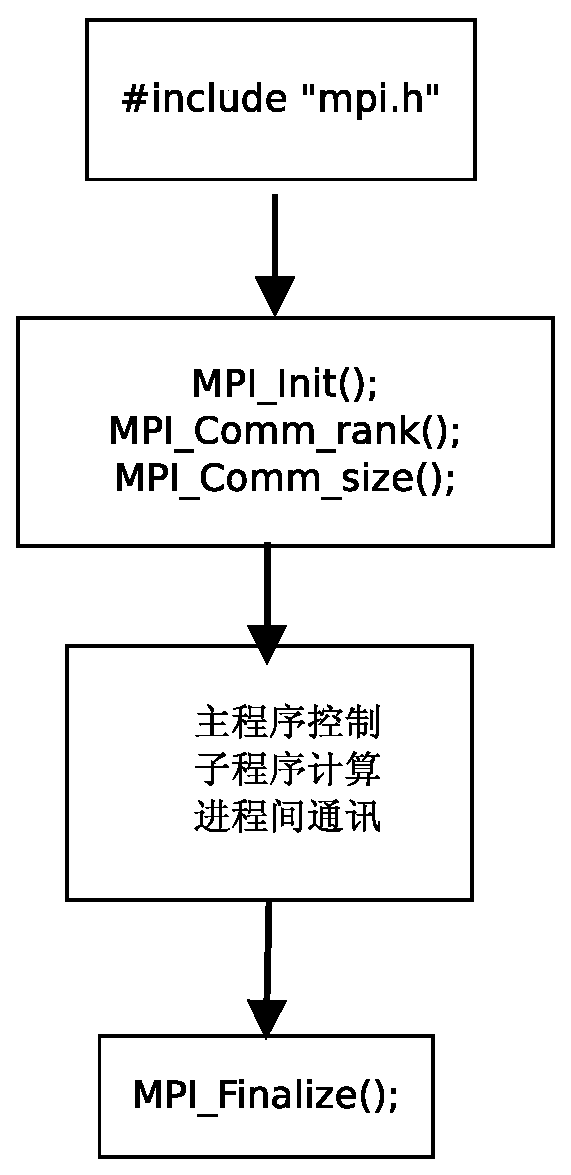
\includegraphics[width=0.3\textwidth]{mpidesignmodel}
    \caption{mpi设计模式}\label{fig:mpidesignmodel}
    \vspace{\baselineskip}
    \end{figure}

\section{MPI编程环境搭建}
     MPI做为消息传递标准,有多种版本的实现,本文和实验都是通过MPICH2来做展开和实验的。MPICH2是Argonne National Laboratory
编写和维护的实现MPI标准的库,MPI由三层架构构成,分别为MPI的API,由点到点通信
和在点到点通信基础上构造的;中间为抽象设备层,用来封装不同的底层通信库的不同接口;底层是具体的底层通信库。MPICH2在保证高性能的
的同时保持了高度的可移植性,支持包括AIX,Linux(IA32,X86\_64),Mac OS/X,Solaris,Windows等多种操作系统平台,同时也做为一个开放
开源的项目。

    本文全部项目采用使用MPICH2作为环境进行实验。以下为系统搭建过程:

    首先准备好系统和网络环境,本文的实验环境为局域网,内有3台装有64位Ubuntu12.04的PC机,CPU为i5-3300,内存为4G,三台机器的
主机名分别为$S1,S2,S3$,其中$S1$作为Server,$S2,S3$作为Worker,PC机上已经装好了Python2.7,SSH,NFS。

\subsection{配置SSH}    
    MPICH2管理分布式计算环境中的各个进程,采用的都是SSH协议,为了方便管理,需要在$S1$上拷贝主机的ssh公钥到$S2,S3$上。 执行
命令:
    \begin{verbatim}
    ssh-keygen -t rsa
    ssh-copy-id -i ~/.ssh/id_rsa.pub root@S2
    ssh-copy-id -i ~/.ssh/id_rsa.pub root@S3
    \end{verbatim}
\subsection{配置NFS}
    需要借助操作系统提供的共享文件系统NFS来在S1和S2,S3之间共享数据。首先在主机S1上建立NFS共享目录:
    \begin{enumerate} 
    \item  创建共享目录:
            
    \begin{verbatim}
             mkdir /share
    \end{verbatim}
    \item  将目录添加到NFS目录中:
    \begin{verbatim}
            修改/etc/exports中添加/share *(sync,rw,no\_root\_squash)
    \end{verbatim}
    \item  开启NFS服务:
    \begin{verbatim}
            service nfs start
    \end{verbatim}
    \item  开启主机S1和S2的挂载目录:
    \begin{verbatim}
           mkdir /share;mount s1:/share /share;mkdir /share mount s1:share /share
    \end{verbatim}
    \end{enumerate}
\subsection{安装MPICH2}
    在主机S1,S2,S3上安装MPICH2
    \begin{enumerate}
    \item 下载最新版本的mpich2.tar.gz,安装c编译器
    \item 解压缩安装包tar zxvf mpich2.tar.gz 
    \item 开始安装
            \begin{enumerate}
            \item cd mpich2  //切换到源代码包文件
            \item ./configure //检测主机配置
            \item make        //编译生成可执行文件
            \item make install //将生成的可执行文件拷贝到系统的路径中去
            \item which mpirun //检测是否安装成功
            \end{enumerate}
    \item 测试本机到其他Linux服务器是否可以通过ssh无密码登录,可以使用ssh user@remotemachine来测试
    \end{enumerate}
    在主机S1创建mpd.hosts文件并加入各个机器的机器名或者对应的ip地址即可

\subsection{MPI环境测试}
    启动MPICH2守护进程:
    \begin{verbatim}
mpdboot -n 1;
    \end{verbatim}

    执行
    \begin{verbatim}
mpdtrace -l,
    \end{verbatim}

执行成功后会得到主机名,监听端口号,主机ip地址。测试成功后mpdallexit退出守护进程。

\subsection{MPI编程}
    MPI编程常见的策略为安装MPI的实现到PC机,进行小数据量测试后,确定程序运行正确之后,进行
并行计算机计算.

    MPI程序的编译和运行方法:
    \begin{enumerate}
    \item 编译MPI代码:C使用mpicxx编译, C++使用mpic++编译
    \item 运行MPI可执行程序:建立进程间联系mpd --ncpus=4 ;运行代码mpiexec -n 4 mpiprogram
    \item 退出MPI可执行程序: mpdallexit
    \end{enumerate}
